\subsection*{Измерения}

Найдём резонансную частоту $f_0$ для образцов. 
% как искать



\begin{figure}[h]
    \centering
    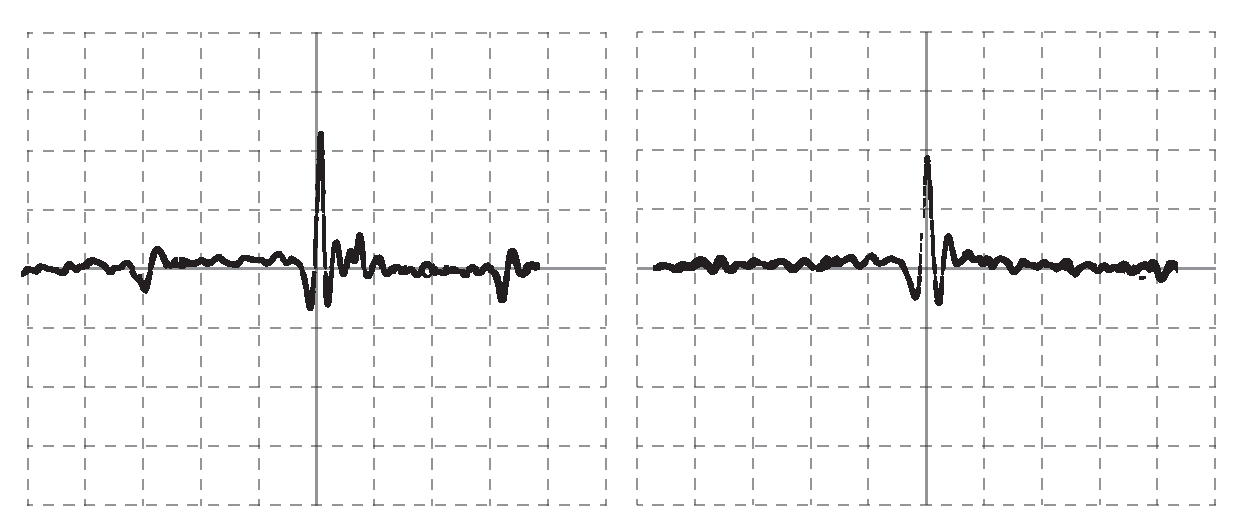
\includegraphics[width=0.5\textwidth]{6.10.4_osc.pdf}
    \caption{Осциллограммы для воды и резины}
    \label{fig:1}
\end{figure}





\noindent
С помощью детектора Холла определим магнитное поле в щели прибора (таблица 1).



\begin{table}[h]
    \centering
    \caption{Измерение $g$-фактора}
    \begin{tabular}{c|ccc|cc|cc|c}
    \toprule
    № & материал & $f_0$, МГц & $B_0$, мТл & $\mu^\text{эксп}$, $\sub{\mu}{я}$ & $\sigma_\mu$, $\sub{\mu}{я}$ & $g^\text{эксп}$ & $\sigma_g$ & $g^\text{таб}$ \\
    \midrule
    1  & резина (H) &  9.805   &  230  & 2.79 & 0.03 & 5.57 & 0.05 & 5.59 \\
    2  & тефлон (F) &  9.800   &  245  & 2.62 & 0.02 & 5.23 & 0.04 & 5.26 \\
    3  & вода   (H) &  9.800   &  230  & 2.79 & 0.03 & 5.57 & 0.05 & 5.59  \\
    \bottomrule
    \end{tabular}
\end{table}

\noindent
Также найдём $g$-фактор и магнитный момент по формулам
\begin{equation*}
    g = \frac{2 \pi \hbar f_0}{\sub{\mu}{я} B_0},
    \hspace{10 mm} 
    \mu = g \sub{\mu}{я} I,
\end{equation*}
где $I = \frac{1}{2}$ для H и F, $\sub{\mu}{я} = 5.05 \cdot 10^{-27} \ \text{Дж}/\text{Тл}$. Занесем полученные результаты в таблицу. 





